% =====================================================================
%  PixelProof - Phase 1 report (anonymous)  -  TSYP14 Track 3
%
%  Build:   python scripts/render_latex.py        (from the repository root)
%
%  The sources use result-file tokens such as {{m:/target_fpr|pct0}}; the script resolves them against results/
%  (and refuses to build if one cannot be resolved) and compiles the copy in build/ with pdflatex.
%  Figures are in figures/. One file per section in sections/.
% =====================================================================
\documentclass[11pt,a4paper]{article}

\usepackage[T1]{fontenc}
\usepackage[utf8]{inputenc}
\usepackage{lmodern}
\usepackage[english]{babel}
\usepackage[margin=2.3cm,headheight=14pt]{geometry}
\usepackage{microtype}
\usepackage{xcolor}
\usepackage{graphicx}
\usepackage{float}
\usepackage{booktabs}
\usepackage{array}
\usepackage{tabularx}
\usepackage{longtable}
\usepackage{multirow}
\usepackage{enumitem}
\usepackage{amsmath}
\usepackage{amssymb}
\usepackage{fancyhdr}
\usepackage{titlesec}
\usepackage{caption}
\usepackage{subcaption}
\usepackage{adjustbox}
\usepackage{listings}
\usepackage[most]{tcolorbox}
\usepackage{tikz}
\usetikzlibrary{arrows.meta,positioning,shapes.misc,fit,calc,backgrounds}
\usepackage[obeyspaces,spaces,hyphens]{url}
\usepackage[hidelinks,pdfusetitle,bookmarksnumbered]{hyperref}

\hypersetup{pdftitle={PixelProof: proving provenance and detecting post-capture manipulation of Earth-observation imagery},
  pdfauthor={},pdfsubject={TSYP14 Track 3 - Phase 1 report (anonymous)},pdfkeywords={provenance, Ed25519, forensics, EuroSAT}}

\graphicspath{{../figures/}{figures/}}
\emergencystretch=2em

% ---------- colours ----------
\definecolor{pxnavy}{HTML}{14325A}
\definecolor{pxblue}{HTML}{2B6CB0}
\definecolor{pxteal}{HTML}{1F9D8B}
\definecolor{pxorange}{HTML}{DD7A1F}
\definecolor{pxred}{HTML}{C0392B}
\definecolor{pxgrey}{HTML}{F1F4F8}
\definecolor{pxline}{HTML}{C9D3E0}
\definecolor{pxgreenbg}{HTML}{E3F4F0}
\definecolor{pxredbg}{HTML}{FBE9E7}
\definecolor{pxbluebg}{HTML}{E6EEF8}
\definecolor{pxorangebg}{HTML}{FDF0E1}

% ---------- sections ----------
\titleformat{\section}{\Large\bfseries\color{pxnavy}}{\thesection}{0.6em}{}
\titleformat{\subsection}{\large\bfseries\color{pxblue}}{\thesubsection}{0.6em}{}
\titleformat{\subsubsection}{\normalsize\bfseries\color{pxnavy}}{\thesubsubsection}{0.6em}{}
\titlespacing*{\section}{0pt}{1.6em}{0.8em}
\titlespacing*{\subsection}{0pt}{1.2em}{0.4em}

% ---------- header / footer ----------
\pagestyle{fancy}
\fancyhf{}
\renewcommand{\headrulewidth}{0.4pt}
\renewcommand{\footrulewidth}{0.4pt}
\fancyhead[L]{\small\color{pxnavy}PixelProof: Trust the Pixel}
\fancyhead[R]{\small\color{pxnavy}Phase 1 Report}
\fancyfoot[L]{\small TSYP14}
\fancyfoot[R]{\small Page \thepage}

% ---------- captions, lists ----------
\captionsetup{font=small,labelfont={bf,color=pxnavy},skip=6pt}
\setlist{itemsep=2pt,topsep=4pt}
\setlength{\parindent}{0pt}
\setlength{\parskip}{5pt}
\renewcommand{\arraystretch}{1.3}
\setcounter{tocdepth}{2}

% ---------- helpers ----------
% \cd{...}: code, file names, paths and identifiers, set in typewriter and allowed to break at / . _ - and spaces.
\urlstyle{tt}
\DeclareUrlCommand\cd{\urlstyle{tt}}
\newcommand{\meas}{\textsc{[measured]}}
\newcommand{\targ}{\textsc{[target]}}
\newcommand{\notmeas}{\textsc{[not measured]}}
\newcommand{\hl}[1]{\textbf{\color{pxnavy}#1}}
% \ext{...}: a value typed in the source because no result file of this repository snapshot holds it
\newcommand{\ext}[1]{#1}
\newcolumntype{L}[1]{>{\raggedright\arraybackslash}p{#1}}
\newcolumntype{Y}{>{\raggedright\arraybackslash}X}

\newtcolorbox{keybox}[1][]{enhanced,breakable,colback=pxgrey,colframe=pxline,boxrule=0.6pt,arc=3pt,
  left=8pt,right=8pt,top=6pt,bottom=6pt,#1}
\newtcolorbox{rubricbox}[1]{enhanced,breakable,colback=pxbluebg,colframe=pxbluebg,borderline west={3pt}{0pt}{pxblue},
  arc=0pt,left=8pt,right=8pt,top=5pt,bottom=5pt,title={},before skip=6pt,after skip=8pt,#1}
\newtcolorbox{warnbox}[1][]{enhanced,breakable,colback=pxorangebg,colframe=pxorangebg,borderline west={3pt}{0pt}{pxorange},
  arc=0pt,left=8pt,right=8pt,top=5pt,bottom=5pt,#1}

\newcommand{\rubric}[2]{\begin{rubricbox}{}\textbf{Rubric: #1.} #2\end{rubricbox}}

% ---------- code listings ----------
\lstset{basicstyle=\ttfamily\scriptsize,breaklines=true,breakatwhitespace=false,columns=fullflexible,
  frame=single,rulecolor=\color{pxline},backgroundcolor=\color{pxgrey},keepspaces=true,
  showstringspaces=false,xleftmargin=2pt,xrightmargin=2pt,aboveskip=6pt,belowskip=6pt,
  keywordstyle=\color{pxblue}\bfseries,commentstyle=\color{gray}\itshape,stringstyle=\color{pxteal},
  literate={->}{{$\rightarrow$}}2}
\lstdefinestyle{py}{language=Python}
\lstdefinestyle{sh}{language=bash}

% ---------- TikZ styles ----------
\tikzset{
  bx/.style={draw=pxblue!70,rounded corners=3pt,fill=white,align=center,font=\scriptsize,inner sep=4pt,minimum height=9mm,text width=22mm},
  bt/.style={bx,draw=pxteal,fill=pxgreenbg},
  br/.style={bx,draw=pxred,fill=pxredbg},
  bo/.style={bx,draw=pxorange,fill=pxorangebg},
  bn/.style={bx,draw=pxnavy,fill=pxnavy,text=white},
  bg/.style={bx,draw=pxline,fill=pxgrey},
  arr/.style={-{Stealth[length=2mm]},draw=pxnavy!70,thick},
  darr/.style={-{Stealth[length=2mm]},draw=pxnavy!60,dashed},
  grp/.style={draw=pxline,dashed,rounded corners=4pt,inner sep=5pt},
  lbl/.style={font=\tiny,text=pxnavy!80}
}

% sections are loaded if present, so the document builds while it is being written
\newcommand{\sect}[1]{\IfFileExists{sections/#1.tex}{\input{sections/#1}}{\typeout{MISSING SECTION #1}}}

% =====================================================================
\begin{document}
\pagenumbering{roman}

% ------------------------------ title page ---------------------------
\begin{titlepage}
\centering
\vspace*{1.2cm}
{\small\color{pxblue}\bfseries TSYP14 Technical Challenge \textperiodcentered{} IEEE \textperiodcentered{} Ground Truth Under Attack\par}
{\small\color{pxblue}\bfseries Track 3: Trust the Pixel\par}
\vspace{1.4cm}
{\fontsize{26}{31}\selectfont\bfseries\color{pxnavy} PixelProof\par}
\vspace{0.5cm}
{\LARGE\bfseries\color{pxnavy} Proving provenance and detecting\\post-capture manipulation of\\Earth-observation imagery\par}
\vspace{0.9cm}
{\large\itshape A cryptographic trust layer and a calibrated forensic detector, with two independent answers kept separate: was the pixel signed, and does the content look manipulated?\par}
\vfill
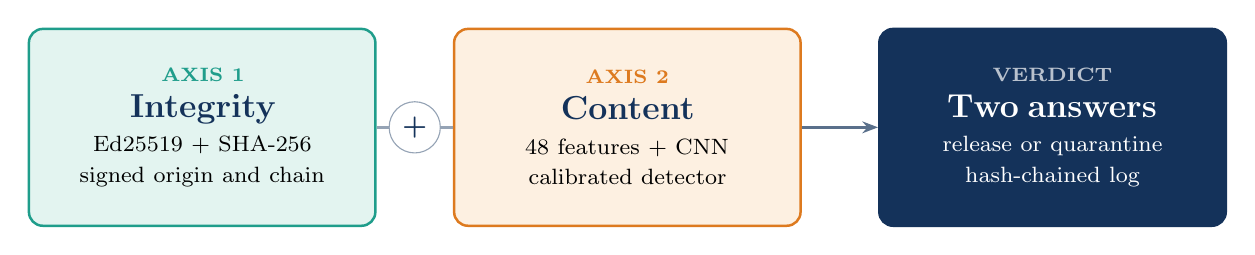
\begin{tikzpicture}[font=\small]
  \tikzset{tb/.style={rounded corners=5pt,minimum width=44mm,minimum height=25mm,text width=40mm,align=center,inner sep=5pt,line width=0.9pt}}
  \node[tb,draw=pxteal,fill=pxgreenbg] (a) at (0,0) {{\scriptsize\bfseries\color{pxteal}AXIS 1}\\[2pt]{\large\bfseries\color{pxnavy}Integrity}\\[3pt]{\footnotesize Ed25519 + SHA-256\\signed origin and chain}};
  \node[tb,draw=pxorange,fill=pxorangebg] (b) at (5.4,0) {{\scriptsize\bfseries\color{pxorange}AXIS 2}\\[2pt]{\large\bfseries\color{pxnavy}Content}\\[3pt]{\footnotesize 48 features + CNN\\calibrated detector}};
  \node[tb,draw=pxnavy,fill=pxnavy,text=white] (c) at (10.8,0) {{\scriptsize\bfseries\color{white!70!pxnavy}VERDICT}\\[2pt]{\large\bfseries Two answers}\\[3pt]{\footnotesize release or quarantine\\hash-chained log}};
  \node[circle,draw=pxnavy!45,fill=white,minimum size=6.5mm,inner sep=0pt,font=\normalsize\bfseries,text=pxnavy] (plus) at (2.7,0) {+};
  \draw[pxnavy!45,line width=0.9pt] (a.east)--(plus.west);
  \draw[pxnavy!45,line width=0.9pt] (plus.east)--(b.west);
  \draw[arr,line width=0.9pt] (b.east)--(c.west);
\end{tikzpicture}
\vfill
{\Large\bfseries Phase 1 Report\par}
\vspace{1.4cm}
\begin{minipage}{0.92\textwidth}
\centering

\includegraphics[height=2.1cm]{logo_cis.png}\hfill

\includegraphics[height=2.1cm]{logo_grss.png}\hfill

\includegraphics[height=2.1cm]{logo_sps.png}
\end{minipage}
\end{titlepage}

% ------------------------------ contents -----------------------------
\tableofcontents
\clearpage
\listoffigures
\clearpage
\listoftables
\clearpage
\pagenumbering{arabic}

% ------------------------------ body ---------------------------------
\sect{01_summary}
\sect{02_scope}
\sect{03_threat}
\sect{04_objectives}
\sect{05_data}
\sect{06_architecture}
\sect{07_trust}
\sect{08_signal}
\sect{09_detector}
\sect{10_scenario}
\sect{11_labs}
\sect{12_dashboard}
\sect{13_feasibility}
\sect{13b_business}
\sect{14_quality}
\sect{15_phase2}
\sect{16_risks}

% ------------------------------ back matter --------------------------
\sect{18_abbreviations}
\sect{19_appendices}
\sect{20_references}

\end{document}
